\chapter{Estrategias de inversión}

\section{Plan de inversión a largo plazo}

Vamos ha estudiar un ejemplo sobre qué activo vamos a trabajar y cómo podríamos hacer este plan de inversión a largo plazo, y cuáles serían las características de este plan de inversión.

El \ti{supuesto básico} es que \tb{la inversión en bolsa en el largo plazo es siempre rentable}, aquí volvemos a un gráfico que ya vimos sobre la evolución de uno de los principales índices que es el \ti{Dow Jones}.

\begin{center}
    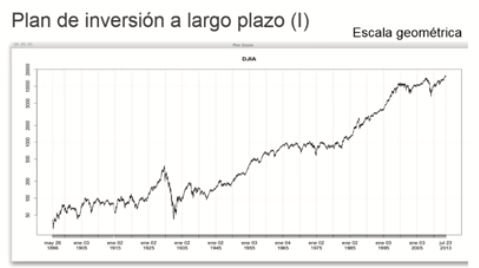
\includegraphics[scale=.85]{images/mod03-01.png}
\end{center}

El gráfico abarca del año 1896 hasta la fecha actual, donde se ve que la inversión en bolsa acaba siendo rentable en el largo plazo.

Apoyándonos en el gráfico podemos señalar:
\begin{itemize}
    \item Si no se eleige el momento de entrada adecuado, puede que tengamos que soportar, durante períodos largos, caídas muy importantes de nuestro capital invertido. Si alguien invirtió a principios de 1929 abría soportado una caída bursátil del \ti{90\%}.
    \item No es bueno invertir todo nuestro capital en un mismo instante de tiempo, lo que proponemos es \tb{periodificar la inversión} durante un período de tiempo, que cuanto más largo sea mejor ratio \ti{rentabilidad-riesgo} nos va a proporcionar.
    \item Introduciremos una nueva medida de riesgo. Vimos que generalmente la medida de riesgo utilizada es la \ti{desviación típica de los rendimientos}; sin embargo, ésta tiene como desventaja que viene medida en un tipo de unidad difícil de entender para el inversor medio o común. Vamos a introducir una nueva medida de riesgo que se conoce como \tb{drawdown}, mide la caída en terminos porcentuales desde un máximo hasta un mínimo entre dos puntos. En el caso expuesto de la caída del $90\%$, si analizamos la rentabilidad obtenida en el largo plazo, y suponemos que realizamos una inversión y que da una rentabilidad del $500\%$, la caída podría representar un $20\%$ dentro de toda esa rentabilidad obtenida. Es decir, para medir el \tb{drawdown} mediremos \ti{la caída en términos porcentuales respecto de la rentabilidad total que se espera obtener de la inversión}.
\end{itemize}

Nos centraremos en el índice Dow Jones, si analizamos su rentabilidad, tenemos el siguiente histograma de rentabilidades anuales para todo el período considerado,
\begin{center}
    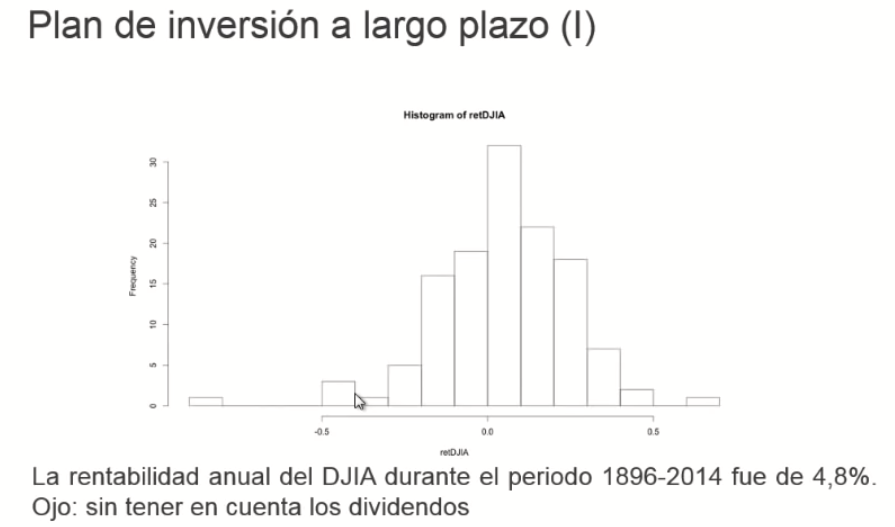
\includegraphics[scale=.65]{images/mod03-02.png}
\end{center}
la rentabilidad anual media ha sido del $4,8\%$, sería la rentabilidad mínima que los inversores deberían haber peido a cualquier inversor bursátil, eso sin tener en cuenta los dividendos, que hemos visto que durante gran parte de la historia han estado por encima del $3\%, 4\% o 5\%$, esa rentabilidad debería añadirse al $4,8\%$.

Si nos centramos, no en todo el período histórico, si no en la franja que va desde 1932, después de la crisis del 29, hasta la actualidad, entonces la rentabilidad ha sido todavía mayor, del $6,7\%$, a lo que añadimos la rentabilidad por dividendos, como mínimo del $3\%$, es fácil ver que la rentabilidad mínima que podríamos obtener sería del $10\%$, que empieza a ser una rentabilidad interesante en el largo plazo.
\begin{center}
    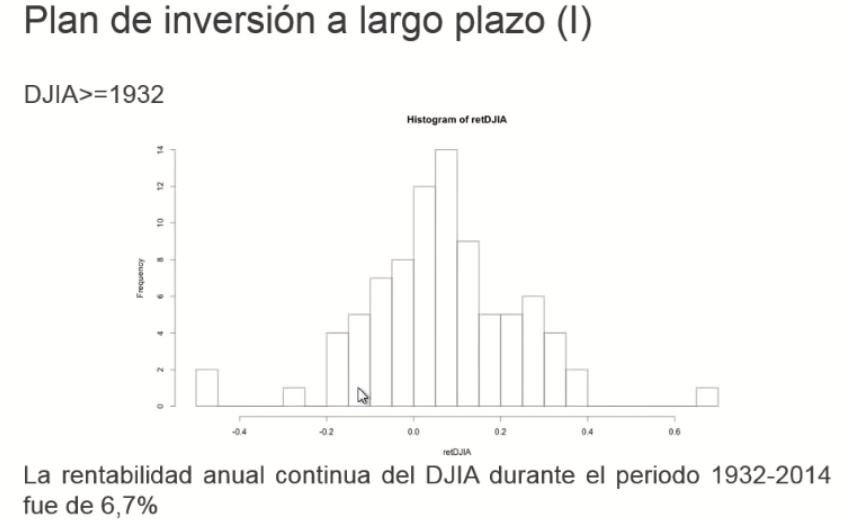
\includegraphics[scale=.65]{images/mod03-03.png}
\end{center}

Analicemos alguna otra cuestión relativa al primer gráfico sobre la evolución del Dow Jones, qué es lo que ocurre si realizamos toda nuestra inversión en un momento determinado de tiempo, si invertimos todo nuestro capital en ese instante de tiempo determinado.
\begin{center}
    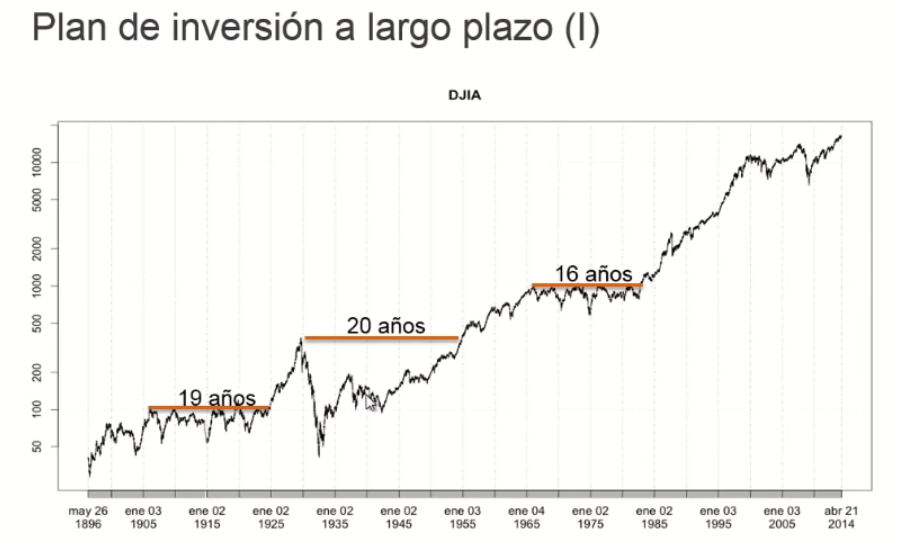
\includegraphics[scale=.65]{images/mod03-04.png}
\end{center}
Puede ocurrir que tengamos que sufrir fuertes caídas en bolsa, de las que tardaremos mucho en recuperarnos. 

Si lo que queremos hacer nuestro propio plan de inversión, y no tener que pagar, por ejemplo, las comisiones, en algunos casos demasidado altas, de los fondos de inversión, es posible que la variable más importante que tenga que ver es cuánto tiempo voy a requerir para recuperarme de alguna de estas caídas.

En la gráfica se nos muestran tres tramos o períodos:
\begin{itemize}
    \item El primero que abarca 19 años, quienes invirtieron al comienzo del mismo, durante ese tiempo tuvieron constantes vaivenes, donde no era ni alcista ni bajista y no pudieron obtener rentabilidad alguna en su inversión. Esto es algo que debemos evitar. Por lo tanto en este tramo no sería la mejor opción invertir el $100\%$ de nuestro capital, deberíamos seguir otra estrategía.
    \item El segúndo tramo está referido a la caída del 29. Quien invirtió en máximos, previos a la caída, tuvo que esperar 20 años para recuperar la inversión, siendo todavía peor que el anterior, ya que soportó una caída del $90\%$.
    \item En el tercer tramo es similar al primero.
\end{itemize}

En conclusión, 
\begin{itemize}
    \item si la inversión se produce en un único instante de tiempo se corre el riesgo de no recuperarla hasta pasado mucho tiempo, tenemos que intentar evitarlo.
    \item el riesgo no se medirá como la \ti{desviación típica} de los rendimientos, sino que utilizaremos una medida que sea más comprensible, el \ti{drawdown}, la caída de máximos en términos porcentuales.
\end{itemize} 

Para evitar estas situaciones:
\begin{enumerate}
    \item La \tb{periodificación de la inversión}, no invertir todo el capital en un único instante de tiempo, si queremos mantener la inversión durante 20 años, repartiremos la inversión durante los 20 años.
    \item La estrategia que seguiremos es invertir una misma cantidad, puede ser de \euros{1.000} o \euros{10.000}, dependerá del capital que cada uno disponga, cada seis meses. Supongamos que $X = 1$ y que dicha cantidad aumenta un $1\%$, incremento que denominamos como \tfun{g}, cada 6 meses.
    
    Eso significa que si invierto \euros{1.000}, dentro de 6 meses tendré que invertir \euros{1.000}+$1\%$ = \euros{1.010}, dentro de 12 meses sería $\euros{1.000}\ast (1,01)^2$, cada seis meses incrementaría esa cantidad en el $1\%$, de tal maner que  si la inversión se prolonga durante 20 años, la última cantidad invertida asciende a $1\ast(1+0,01)^{39} = 1,47$, si invierto inicialmente \euros{1.000}, la última aportación a la inversión será de \euros{1.470}.
    \item Finalmente, durante ese período de tiempo ¿cuánto habré invertido?, para ello utilizamos la siguiente fórmula:
    $$S = X \ast ((1 + g)^{\text{per}}-1)/g = 1\ast ((1+0,01)^{40}-1)/0,01 = 48,886$$
    Nuestro objetivo es que al final de los 20 años, la cantidad que recuperemeos sea mayor de esos \euros{48,886}. Si queríamos obtener una rentabilidad superior al $10\%$, la cantidad final deberá ser muy superior a los \euros{48,886}.
\end{enumerate}

Hemos visto que importe tendríamos que invertir cada 6 meses durante 20 años, inversión a largo plazo. Terminariamos invirtiendo \euros{48,886}, teniendo en cuenta que \ti{X = \euros{1}}, el importe final tendríamos que multiplicarlo por la cantidad con la que queremos comenzar la inversión, si ésta es de \euros{1.000}, la inversión final sería de \euros{48.886}. Lo que queremos saber es, ¿esos \euros{48.886} en cuánto acaban convirtiéndos para poder calcular la rentabilidad?.

Veamos que rentabilidades habríamos obtenido si la inversión se hubiera realizado sobre el índice Dow Jones.

\begin{center}
    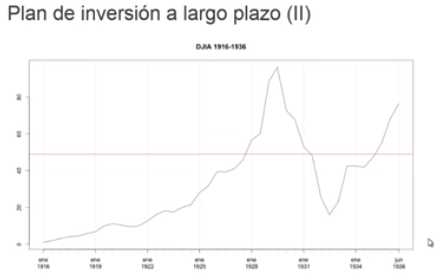
\includegraphics[scale=.65]{images/mod03-05.png}
\end{center}
En el gráfico se puede analizar la evolución durante el período 1916-1936, la primera cantidad la invertiremos en el primer semestre de 1916, y la última el último semestre de 1936. La línea roja representa la cantidad que finalmente estamos invirtiendo, los \euros{48,886}. Se observa que conforme pasa el tiempo la inversión aumenta su valor hasta un punto máximo en el que comienza una caída abrupta, que coincide con la crisis del 1929. Cuando toca fin la caída comienza una nueva recuperación, hasta el último semestre del 1936 donde se sitúa en torno a las setenta y cinco unidades.

¿Cuál habría sido la rentabilidad obtenida?. Habríamos invertido casi cincuenta unidades (\euros{48,886}) y acabamos obteniendo setenta y cinco unidades, lo que significa que estamos teniendo una rentabilidad del $50\%$ sobre la inversión realizada. El \ti{«pero»} sería que hemos sufrido la mayor crisis bursátil de la historia, lo que ha disminuido nuestro rendimiento, aún así se comprueba que no sólo se recupera lo invertido, sino que obtenemos una rentabilidad del cincuenta por ciento, uqe no está nada mal dada las circunstancias.

Tenemos que analizar que ocurre con otros períodos de veinte años. Por ejemplo, qué ocurre si iniciamos la inversión en el año 1926 y la finalizamos en el 1946,

\begin{center}
    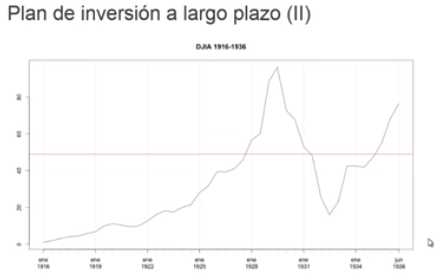
\includegraphics[scale=.65]{images/mod03-05.png}
\end{center}
Vemos que el período analizado terminaría con una rentabilidad entorno al ochenta por ciento, una rentabilidad superior a la vista del cincuenta por ciento anterior. De nuevo hemos padecido la crisis del año 29, y lo más importante, lo que tardamos en recuperarnos de esa crisis, sólo en 4 años hemos recuperado el capital, y eso debido a seguir la estrategia de la \ti{períodicidad de la inversión}.

Otro período de veinte años sería el que va de 1936 a 1956, aquí ya no le afecta directamente la crisis bursátil del 29.

\begin{center}
    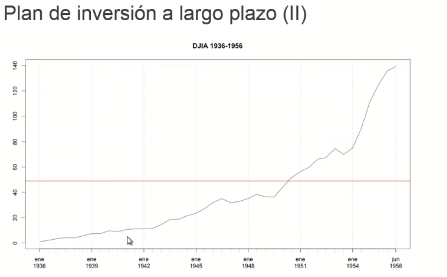
\includegraphics[scale=.65]{images/mod03-07.png}
\end{center}
Se observa como apenas hay caídas y nuestra inversión casi contínuamente hasta case ciento cuarenta unidades, prácticamente multiplicamos por tres lo invertido, estamos hablando de una rentabilidad en torno al $200\%$. 

Algo parecido ocurre con el período 1946 a 1976.

\begin{center}
    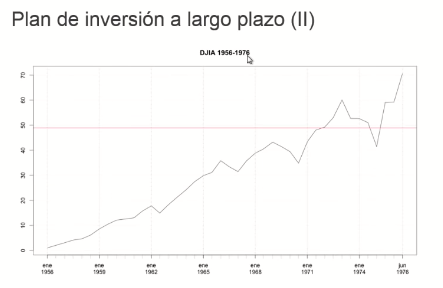
\includegraphics[scale=.65]{images/mod03-08.png}
\end{center}
Aquí la rentabilidad es menor, entorno a las setenta unidades. En sucesivos périodos tenemos más o menos los mismos resultados, y pasamos a ver la última serie, la que abarca los años 1993 a 2014.

\begin{center}
    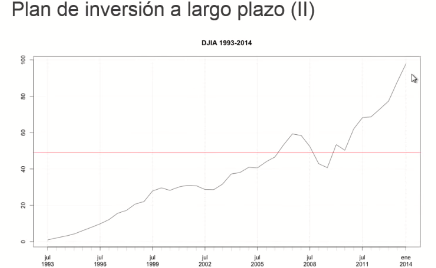
\includegraphics[scale=.65]{images/mod03-09.png}
\end{center}

Resumiendo, en ninguno de estos casos se finaliza perdiendo dinero, y por lo general, la rentabilidad mínima ronda el 50\%, siguiendo la estrategia que no requiere dedicación de tiempo, sino una estrategia  a largo plazo donde cada seis meses invertimos la misma cantidad. Esta sería la estrategia adecuada para personas cuya actividad profesional no está ligada a la bolsa, pero quieren rentabilizar su capital dedicándole un esfuerzo mínimo.

Qué ocurre si observamos la evolución de esta estrategia, empezando la inversión en el año 1916, 1917, 1918, 1919, etc. esto nos permitiría tener muchísimos más períodos de 20 años contemplados, y los resultados obtenidos serían más consistentes, no se podría decir que se deben al azar.

Esto es lo que hemos hecho, hemos observado los subperíodos de 20 años desde 1916 a 2014 para el DJIA, y su representación en un histograma sería

\begin{center}
    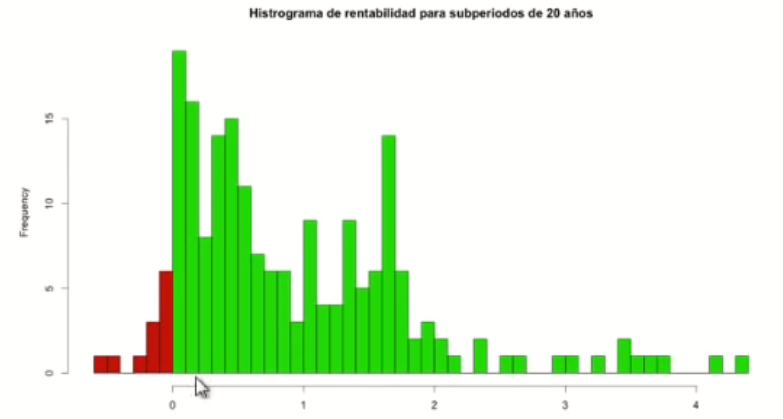
\includegraphics[scale=.65]{images/mod03-10.png}
\end{center}
En rojo están los períodos en los que se pierde rentabilidad, perdemos capital, en verde aquellos períodos en los que la rentabilidad es positiva; el 1 indica que obtenemos una rentabilidad del 100\%, el 2 del 200\% y así sucesivamente. En el histograma se observa que el 94\% de los subperíodos obtuvieron una rentabilidad positiva, sin tener en cuenta los dividendos, es decir, la probabilidad de \tb{no obtener rentabilidad del capital inicial invertido} es sólo del 6\%, el 94\% obtendremos rentabilidades positivas.

Si consideramos los dividendos, que por ejemplo tuviran una rentabilidad media del 4\% por dividendo,

\begin{center}
    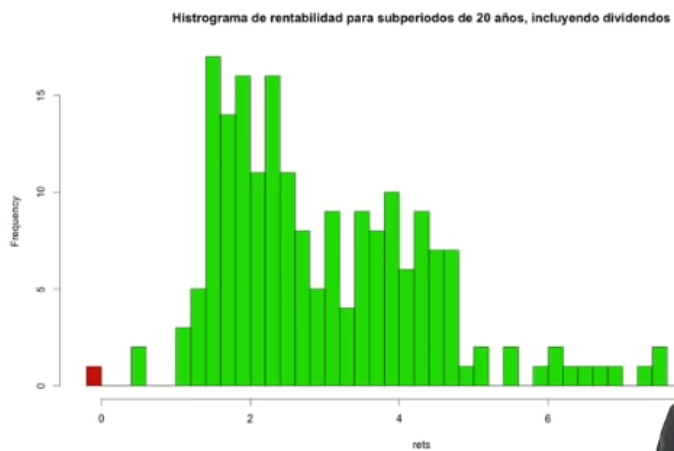
\includegraphics[scale=.65]{images/mod03-11.png}
\end{center}
Vemos que sólo un subperíodo obtiene una rentabilidad negativa, 0,5\% de los casos, la probabilidad de ganar dinero en el largo plazo sería del 99,5\%, podemos asegurar que prácticamente nuestra revalorización está asegurada y es de aproximadamente un 300\%, es decir, estaría multiplicando por 4 el capital inicial.

\section{Estrategias de trading}

Hasta ahora hemos vistos estrategias a seguir por el inversor pasivo, aquél que quiere cubrirse del efecto negativo que puede tener la inflación sobre sus ahorros, su capital. 

A continuación analizaremos posibles estrategias a utilizar por aquellos inversores que quieren hacer \tb{tradding}, algo más agresivo, no se trata del largo plazo, sino un tradding a \tb{medio plazo} o a \tb{corto plazo} e incluso \tb{intradía}.

\subsection{Estrategia de Bandera (flag)}

Basaremos nuestra estrategia de inversión en la \ti{identificación y utilización de figuras técnicas, la \tb{bandera}}.

Lo que nos interesa es ver si al aplicar la estrategia sobre diferentes tipos de activos, de time frames o ventanas temporales obtenemos finalmente una rentabilidad positiva, sostenible en el largo plazo, y  si es posible con el mínimo riesgo posible.

En la actualidad, se estima que aproximadamente el 75\% de las operaciones diarias que llevan a cabo los \ti{mercados financieros} son realizadas por \ti{aplicaciones de programas}, lo que se conocen como \tb{robots}. Es decir, el \ti{tradding algorítmico} gana cada vez más peso y se basa en:
\begin{itemize}
    \item La idea de aplicar estas estrategias.
    \item Validarlas a través de algún paquete informático sobre diferentes activos y ventanas temporales, para tener la seguridad de que esa estrategia funciona y lo hace bien.
\end{itemize}

En nuestro caso bamos a desarrollar un estrategia basada en la figura conocida como \tb{flag (bandera)}. Básicamente \ti{flag} consiste en una ruptura brusca del precio que es seguido por un período en el cual el precio se mantiene con menos volatilidad, dentro de un rango determinado. Eso augura un nuevo movimiento abrupto del precio que es el que intentaremos aprovechar a través de esta estrategia.

Veamos como aplicar esta estrategia siguiendo una serie de pasos.

\begin{center}
    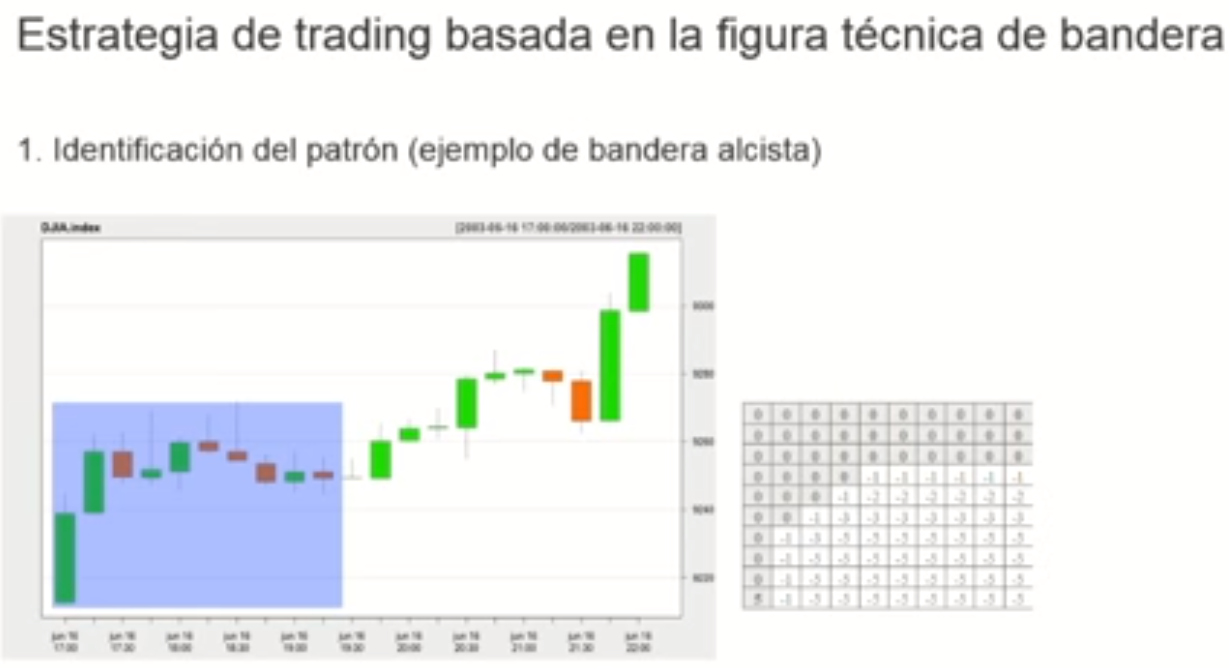
\includegraphics[scale=.45]{images/mod03-12.png}
\end{center}

\begin{enumerate}
    \item Identificar el patrón. Hemos dicho que básicamente la bandera  refleja un movimiento abrupto del precio. En el gráfico, zona sombreada, vemos que la primera bandera representa un movimiento alcista, el precio sube con fuerza, de repente se separa, se mantiene dentro de un rango determinado, con subidas y bajadas (zona sombreada), y lo que esperamos es que siga la tendencia alcista, el momento en el que el precio vuelve a romper hacia arriba. Esta zona sombreada sería la identificación del \ti{patrón bandera}, en nuestro caso sobre el índice DJIA. Además, estamos trabajando sobre datos de quince minutos, cada una de las velas se corresponde con el movimiento de precio en quince minutos.
    
    ¿Cómo identificamos las banderas?. Podemos hacerlo visualmente, pero si lo que queremos es analizar esta estructura y plantear una estrategia y aplicarla sobre una ventana temporal, hay que automatizar la identificación del patrón. En nuestro caso, lo que se hizo fue desarrollar una \ti{matriz de pesos} que se superpone sobre la ventana de precios

    \begin{center}
        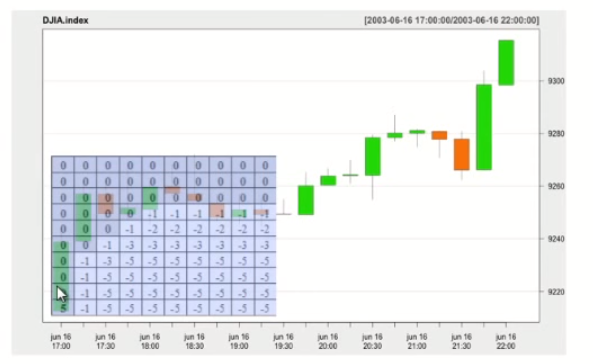
\includegraphics[scale=.65]{images/mod03-13.png}
    \end{center}
    Lo que se intenta es que los precios caígan sobre las celdas que aparecen etiquetadas como cero. Si hay algún precio que se sale de esta zona, cayera por la zona inferior de la tabla, menos sombreada, entonces no identificariamos ese movimiento con el correspondiente patrón bandera. Aquí vemos como el precio rompe hacia arriba, se mantienen las celdas que aparecen con valor 0, y hay tres celdas que aparecen con valor de -1, es decir, \ti{no sería una banderea perfecta} que puedieramos identificar de manera inequivoca, pero sí se acercaría bastante al haber sólo tres celdas que incumplen la propiedad. Seamos permisivos e identifiquemos esta situación como \ti{patrón bandera}, sería una \ti{bandera alcista}, la ruptura del precio se ha hecho hacia arriba, alcista, ha entrado en un rango en el lateral, y lo que intuimos es que el precio va a romper hacia arriba. Lo que haríamos en este caso es tomar una \ti{posición larga}, compraríamos el activo DJIA, en el punto anterior a la primera vela que sale de la matriz de pesos.

    \item Ya hemos identificado un \ti{patrón bandera}, lo que hacemos es iniciar la operación, marcando los niveles de \tb{stop loss} y de \tb{take profit}. Estos dos conceptos, básicamente ayudan a realizar una gestión monetaria correcta:
    \begin{itemize}
        \item \tb{take profit}, nos marca el nivel de beneficio que aspiramos a tener en la operación.
        \item \tb{stop loss}, marca la pérdida máxima que estamos dispuestos a asumir.
    \end{itemize}
    Si el precio evoluciona a nuestro favor cerraremos la operación una vez que el precio haya alcanzado el nivel marcado para el \ti{take profit}, si el precio va en nuestra contra, hemos comprado en largo y de repente el activo empieza a caer, cerraremos la operación en el nivel de \ti{stop loss} que hayamos marcado y, simplemente, asumiremos la pérdida.
    \begin{center}
        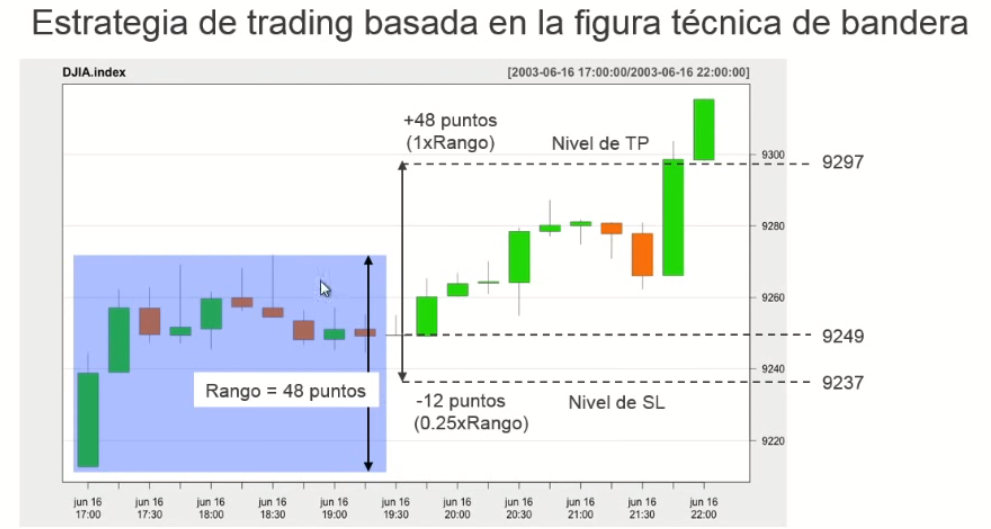
\includegraphics[scale=.65]{images/mod03-14.png}
    \end{center}
    En este caso, dentro de la ventana de 10 velas (zona sombreada gris), tuvo un rango de 48 puntos, es decir, la diferencia entre el máximo del precio y el mínimo. 

    Nosotros, lo que hacemos es marcar un \ti{take profit} que tenga ese mismo rango de puntos. Si compramos en un nivel de 9249 puntos, le sumamos 48 y esa será la cantidad de nuestro \ti{take profit} = 9297 puntos, estamos tomando como \ti{take profit} 1 por el rango (48 puntos). ¿Cuánto corresponde al \ti{stop loss}?. Hay una regla básica en el análisis técnico que nos dice que el \ti{stop loss} debería ser lo más bajo posible y siempre inferior al \ti{take profit}, es decir, si quiero una rentabilidad de 48 puntos, la máxima pérdida que esto dispuesto a soportar tiene que ser inferior a 48. En este caso hemos considerado una cuarta parte del rango (48/4 = 12), el ratio es de 4 a 1. Por lo tanto, si compramos el índice en 9249 puntos, le restariamos 12 y obtendríamos un \ti{stop less} de 9237. Si el precio baja hasta esta posición, cerramos la posición y asumimos una pérdida de 12 puntos.

    En este caso, lo que ocurrió es que el precio fué hacia arriba hasta que llegó al nivel marcado como \ti{take profit}, por lo que el beneficio de esta operación habría sido de 48 puntos. La operación se habría abierto a las 19:15 o 19:30 y la habríamos cerrado a las 21:45, se trataría de una operación \ti{intradía}.
    \item Esta estrategia debe aplicarse ahora sobre diferentes índices bursátiles como DJIAX, DAX, FTSE, IBEX y sobre diferentes pares de divisas: EUR-USD, USD-JPY, USD-CAD, USD-AUD; esto se hace para ganar consistencia, para ver que efectivamente esta estrategia de trading funciona, no sólo para un activo, sino para otros índices y diferentes pares de divisas. Se aplicará no sólo sobre velas de 15 minutos, sino también sobre velas de 1 hora, 4 horas e incluso velas diarias.
    
    Lo que necesitamos, para validar una estrategia, es el mayor número de observaciones posibles, en nuestro caso lo que hicimos fue analizar el DJIA desde el 22 de mayo del 2000 hasta el 29 de novimbre e 2013, utilizamos velas de 15 minutos, lo que supone que el trabajo de validación de estrategias se hizo sobre un total de 91.300 velas, aquí si contamos con una base de datos muy amplia y por lo tanto los resultados que se obtengan tienen validez estadística. 

    También se hicieron cambios en los valores de \ti{stop less} y de \ti{take profit} para saber exactamente con qué configuraciones la estrategia resultaba más rentable.

    \begin{center}
        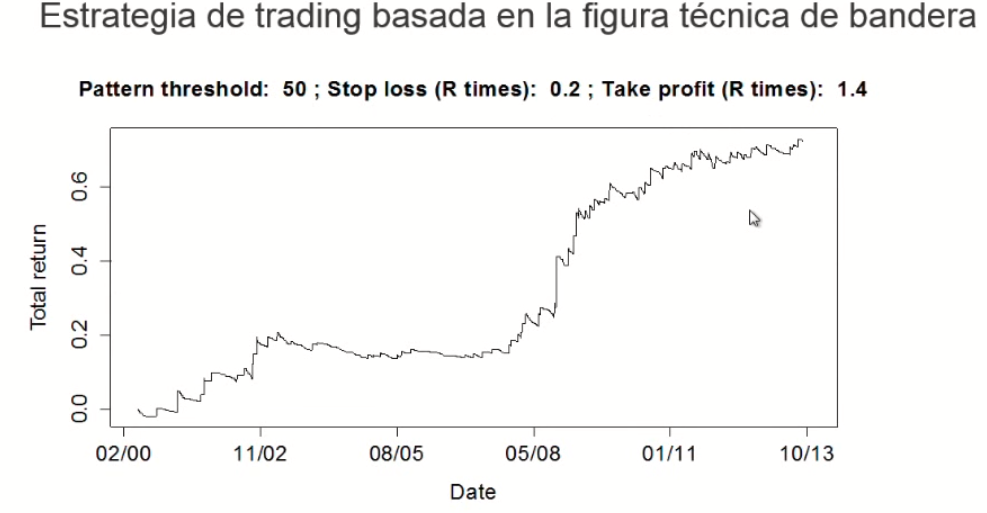
\includegraphics[scale=.65]{images/mod03-15.png}
    \end{center}
    Vemos la curva de rendimiento que obtendríamos al aplicar la estrategia del patrón bandera sobre el DJIA, desde el año 2000 hasta el 2013, tomamos un \ti{stop less} que suponía un 20\% del rango (multiplicar el ranco por 0.2) y un \ti{take profit} de \ti{1.4}, el ratio beneficio-riesgo era de 7:1. Lo que vemos es que la regla de trading o estrategia bursátil acaba siendo rentable y, realmente, las pérdidas que asumimos durante todo el período de tiempo, el \ti{drawdonw}, el riesgo, es relativamente pequeño. Vemos que las bajadas son relativamente pequeñas frente al beneficio obtenido finalmente.

    Si cambiamos\footnote{Además del stop loss y el take profit se cambia el \ti{pattern threshold}, que no se ha explicado para no alargar el vídeo.} el \ti{stop loss} y el \ti{take profit}, para analizar la robustez de la estrategia:
    \begin{center}
        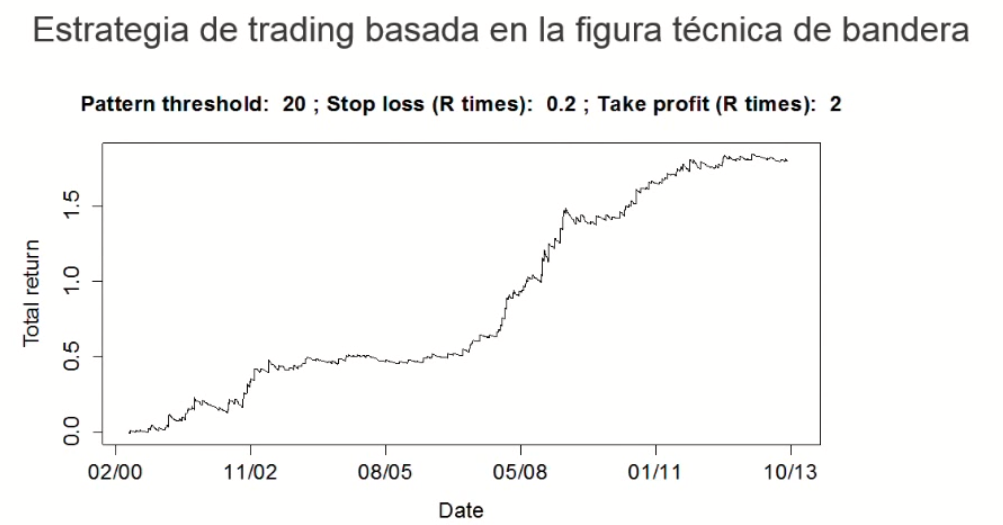
\includegraphics[scale=.65]{images/mod03-16.png}
    \end{center}
    vemos que la estrategia sigue siendo rentable, además es la mejor de las configuraciones, donde el \ti{stop loss = 0.2} y el \ti{take profit = 2}, con una rentabilidad cercana al 200\%, y el drawdown representa un porcentaje realmente pequeño, no va más allá de un 10 al 15 por ciento frente al casi 200 por cien de la rentabilidad.
\end{enumerate}

Podemos comparar esta estragia con una estrategia pasiva de gestión pasica, comparar el índice en el año 2000 y venderlo en el 2013.
\begin{center}
    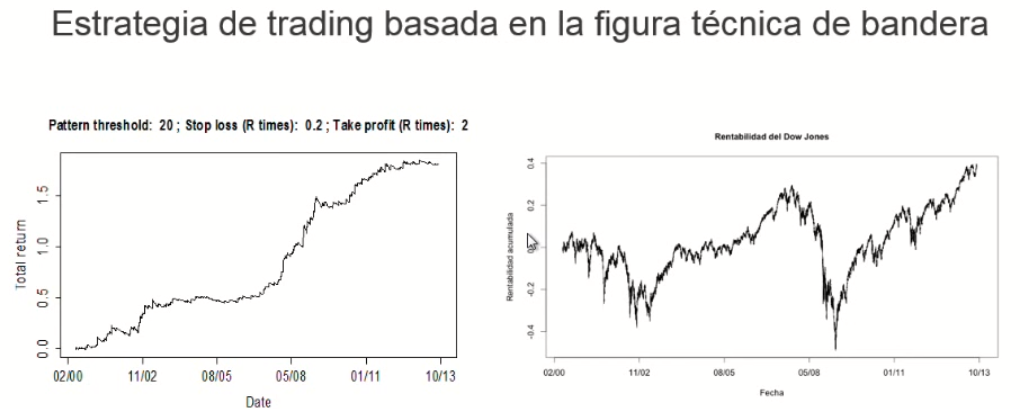
\includegraphics[scale=.65]{images/mod03-17.png}
\end{center}
Si hubieramos realizado esa operación la rentabilidad habría sido del 40\%, habríamos obtenido una rentabilidad inferior a la de la estrategía activa, pero aún más importante el riesgo que estamos asumiendo, \ti{drawdown}, es mucho mayor. En el gráfico de la derecha, vemos como el índice, que aproximadamente es el año 2008, iba ganando un 30\% respecto del 2000, llegó a bajar hasta un -50\%, tenemos un \ti{drawdown} de un 80\%, si al final ganamos un 40\% estamos asumiendo el doble de riesgo que beneficio vamos a obtener.

Esto nos da la idea de que nuestra estrategia de gestión activa es mejor que la correspondiente a la gestión pasiva.

Vamos a estudiar una cuestión muy interesanete, la \tb{correlación entre el stop loss y el take profit y la rentabilidad media y el riesgo medido mediante el drawdown}. Para ello lo que se plantea es una \ti{matriz de correlaciones} entre todas las variables que configuran la estrategia.
\begin{center}
    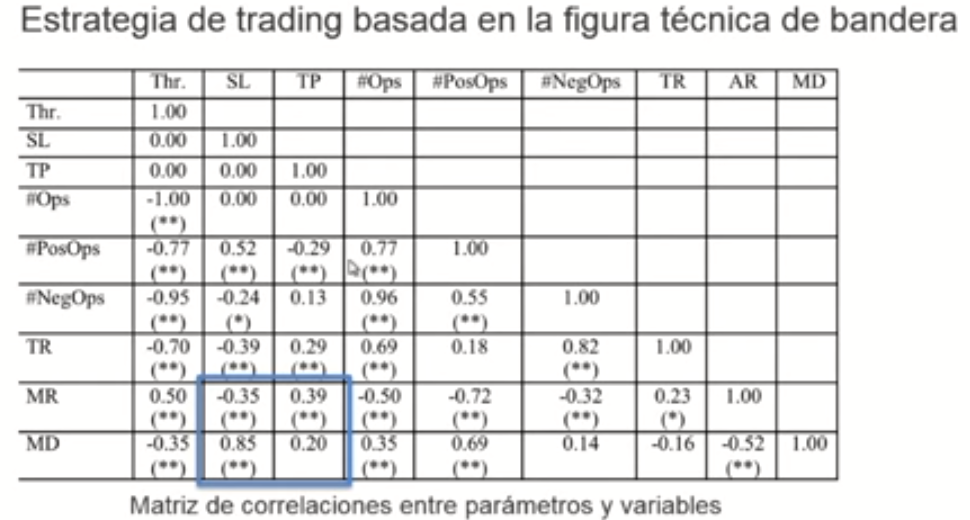
\includegraphics[scale=.65]{images/mod03-18.png}
\end{center}
La \ti{correlación es un estadístico} que sirve para medir la dependencia o la relación lineal que existe entre dos variables. La correlación va desde -1 a +1, de tal manera que:
\begin{itemize}
    \item Si dos variables tienen una correlación próxima a +1, significa que las dos tienen una relación directa y fuerte; es decir, cuando una sube, la otra también, y lo mismo cuando se produce una bajada.
    \item Si la correlación es negativa y próxima a -1, existe una relación inversa, es decir, cuando una variable sube, la otra baja y viceversa.
\end{itemize} 

En el caso remarcado en la imagen de la matriz, se reproduce el segundo caso, que pasamos a analizar la que obtuvo, en valor absoluto, un coeficiente mayor representada por la \ti{correlación entre el máximo drawdown (MD)}, la medida de riesgo, y el \ti{stop loss (SL)} que nos habíamos marcado. Vemos que la \ti{correlación es positiva} y está \ti{próxima a +1}, es de \ti{0.85}, esto significa que cuanto mayor sea el \ti{stop loss} mayor va a ser el \ti{drawdown} en nuestra estrategia, por lo tanto, lo que conviene es ceñir ese \ti{stop loss} lo más bajo posible, por ejemplo $0.2$ veces el rango, para así disminuir el riesgo.

Si analizamos la \ti{correlación entre rentabilidad media (MR) o rentabilidad por operación, niveles de stop loss (SL) y take profit (TP)} vemos que la correlación con el \ti{stop loss} es \tb{negativa}, cuanto más grande sea el \ti{stop loss} menor va a sr la \ti{rentabilidad por operación} que se obtenga, mientras que conforme aumenta el nivel de \ti{take profit} mayor va a ser también la \ti{rentabilidad por operación}, es decir, podemos aplicar esta misma estrategia, pero siempre será más interesante alargar lo máximo posible el \ti{take profit} porque eso conseguirá que la \ti{rentabilidad por operación}, sea mayor y, por lo tanto, la \tb{rentabilidad total} también lo sea.
\begin{center}
    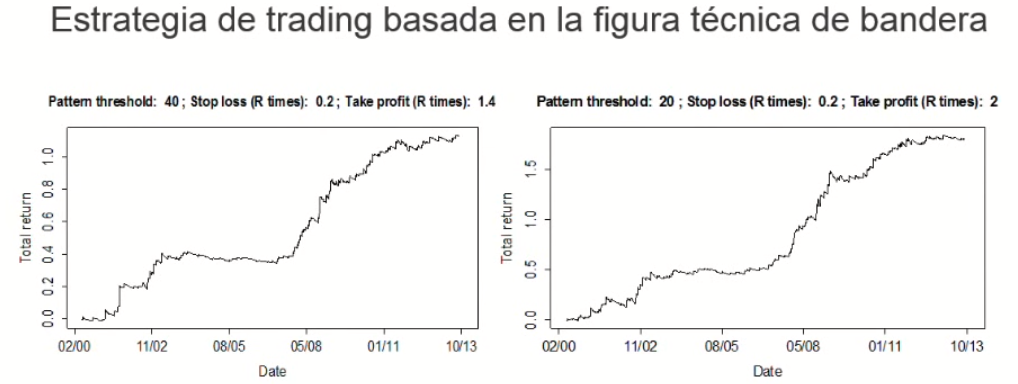
\includegraphics[scale=.65]{images/mod03-19.png}
\end{center}
En el gráfico se compara la misma estrategia pero con dos configuraciones distintas.
\begin{itemize}
    \item La primera tiene un \ti{stop loss = 0.2} y un \ti{take profit = 1.4} veces el rango.
    \item La segunda mantiene el mismo \ti{stop loss}, pero un \ti{take profit = 2} veces el rango.
\end{itemize}
Lo que observamos es lo que nos indicaba la matriz de correlaciones, cuanto mayor es el \ti{take profit} mayor es la \ti{rentabilidad media por operación}, y por lo tanto la \ti{rentabilidad total}. En el segundo caso, la rentabilidad está próxima al 200\%, mientras que en el primer caso, la rentabilidad está un poco por encima del 100\%, prácticamente podemos doblar la rentabilidad total simplemente pasando de un \ti{take profit} de .4 a 2.

\subsection{Estrategia basada en el Indicador de Media Móvil}

Una estrategia que históricamente ha sido rentable en el pasado, puede llegar un momento en el que deje de serlo. En ocasiones esto ocurre porque hay avances tecnológicos, o porqu esa estrategia se vuelve tan popular, y es utilizada masivamente, que todo el mundo acaba haciendo lo mismo y, al final, nadie obtiene rentabilidad. Vamos a ver un ejemplo de ésto, una estrategia que ha dejado de funcionar.

Esto implica que los traders, los inversores,  sobre todo los que se dedican más al medio y corto plazo tienen que estar permanentemente validando sus estrategias, incorporando nuevos indicadores o aspectos para mejorar dichas estrategias.

La estrategia que analizamos está basada en el \ti{cruce d dos medias móviles}, una media móvil larga y otra corta, una rápida y otra lenta.
\begin{center}
    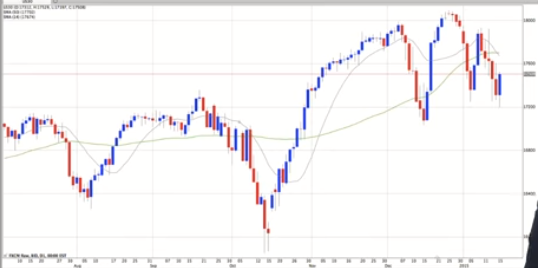
\includegraphics[scale=.65]{images/mod03-20.png}
\end{center}
El ejemplo esta referido a los datos del Dow Jones, trabajamos con datos o con velas diarias, cada una de estas velas representa la evolución de la cotización de un día, y lo que hemos representado han sido dos medias móviles:
\begin{itemize}
    \item Una media móvil lenta, la de 50 períodos, línea de verde más oscuro.
    \item Una media móvil rápida de 14 períodos, algo más clara.
\end{itemize}
Lo que dice esta estrategia es qué posición debemos tomar en el mercado largo o cortos, comprar o vender, en función del punto de cruce de las medias.
\begin{itemize}
    \item Cuando la media rápida cruza a la media lenta, hacia abajo (primer cruce en la parte izquierda de la imagen), sería una \tb{señal de venta}, deberíamos vender el activo. Observamos como sigue evolucionando el precio.
    \item El siguiente cruce, la media rápida se cruza con la lenta en un momento de alza, sería una \tb{señal de compra}, aquí sería conveniente comprar y mantener las compras hasta que de nuevo se produzca un cruce descendente.
\end{itemize}
En el gráfico vemos que durante el período analizado tendríamos \ti{cinco cruces}, es decir, \ti{cinco operaciones de compra y venta}, que puede que fueran rentables o no. De nuevo debemos considerar un horizonte temporal más amplio para extraer conclusiones.

Este tipo de estrategias ha sido  muy estudada y aquí recopilaremos los resultados de dos de estos trabajos académicos. 

\begin{itemize}
    \item El primero se publicó en 1992 en \ti{The Journal of Finance}
    \begin{center}
        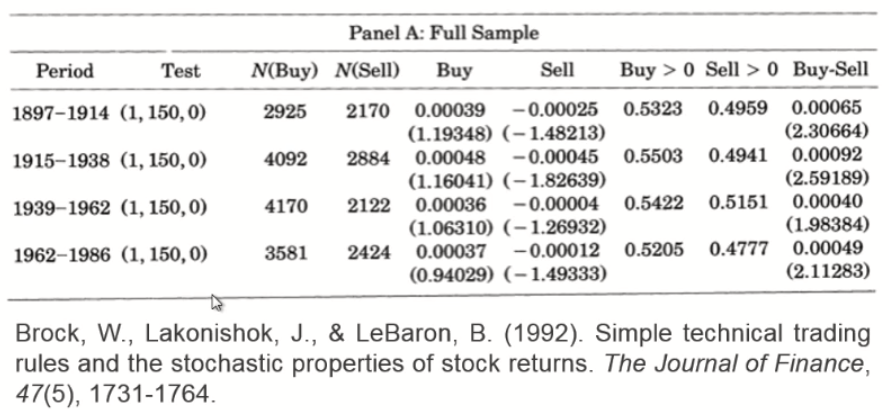
\includegraphics[scale=.65]{images/mod03-21.png}
    \end{center}
    Lo que hicieron fue analizar el Dow Jones durante un período histórico muy largo, desde 1897 hasta 1986, y aplicaron estrategias basadas en el \ti{cruce de medias móviles} sobre todo el período completo para evaluar si se obtenía o no, una rentabilidad positiva. Para el período completo observarón que sí, era rentable. Fueron un poco más ayá e indicarón que era posible que la estrategia funcionara muy bien durante todo el período, porque puede funcionar bien en un período determinado y el resto no dar beneficio ni pérdidas, sino que se mantiene estable durante todo el período. 
    
    Para contrastar esto lo que hicieron fue dividir el período completo en cuatro subperíodos, aplicar la estrategia para cada uno de ellos, obtiendo que la estrategia era igualmente rentable para cada uno de ellos.
    \item En 1999 aparece un nuevo trabajo, en la misma revista, en el que los autores utilizaban el mismo índice, aplicando la misma estrategia y los mismos parámetros para el período 1987-1996. Lo que descubrieron es que durante toda esa década la estrategia ya había dejado de ser rentable, por lo tanto, algo que sí había funcionado bien históricamente en el pasado, apartir de ahí (1987) dejó de funcionar.
\end{itemize}
La conclusión es que efectivamente podemos tener o leer estrategias en libros o análisis clásicos sobre trading, que en el pasado pudieron funcionar muy bien, pero que es posible que ahora estén obsoletas.

Sin embargo, es posible que muchas de ellas se puedan adaptar, mejorar y combinar diferentes indicadores, osciladores o figuras técnicas chartistas de tal manera que sigan siendo rentables en la actualidad. Es lo que nosotros pretendemos en esta sección.

Vamos a presentar un ejemplo en el que únicamente vamos a utilizar el precio y la media móvil, una media móvil de 200. El índice que analizamos es el DAX-30 (índice Alemán), son datos de quince minutos, cada vela representa quince minutos, cada uno de los rectángulos de fondo representan un día. La media móvil está representada por la línea contínua superior, y vemos que el precio siempre está por debajo de la media móvil, estaríamos ante un escenario bajista.
\begin{center}
    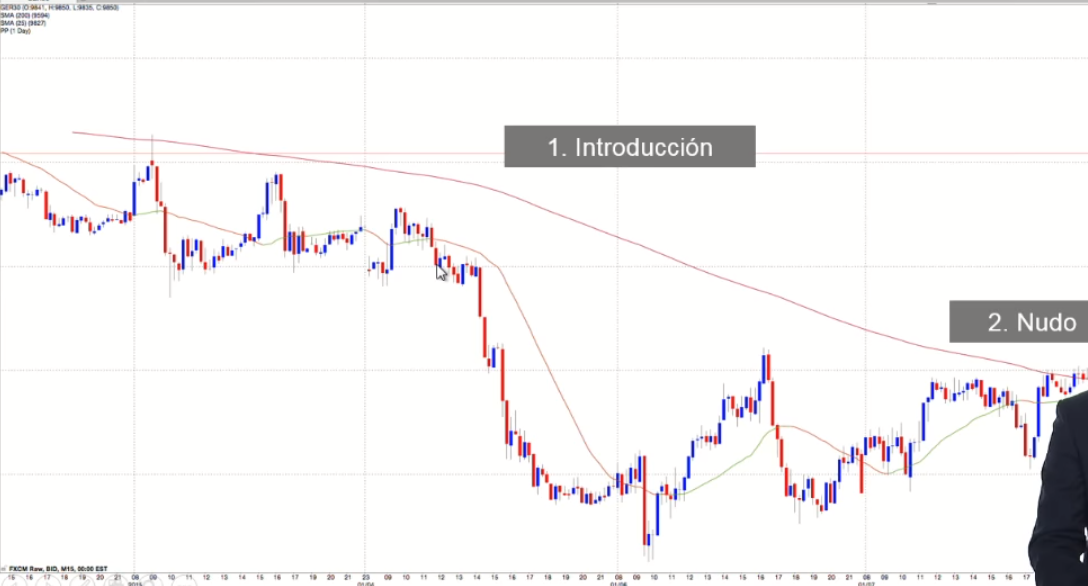
\includegraphics[scale=.65]{images/mod03-22.png}
\end{center}
Vemos, en la parte izquierda, como el precio llegó a tocar la media móvil, pero esta lo había rechazado, y el precio se fue hacia abajo.

Analizaremos el ejemplo en tres fases:

\begin{itemize}
    \item \tb{Introducción}. Vemos que son dos los personajes que intervienen en este esquema:
    \begin{itemize}
        \item el precio.
        \item la media móvil
    \end{itemize}
    Existe un equilibrio entre ellos, el precio en todo momento está por debajo de la media móvil, la situación de equilibrio es la del mercado. bajista.

    Lo que se observa en el rectángulo correspondiente al cuarto día, es que el precio se aproxima a la media móvil, se prueba si es posible una reacción alcista, parte de la reacción es previa, donde el precio dejó de bajar y ha estado subiendo con oscilaciones.
    \item \tb{Nudo}. Aquí el equilibrio se rompe.  Lo que hay que ver es si será capaz de romper esa media móvil hacia el alza y, por lo tanto, sería bueno comprar el activo y entrar en largos, o si finalmente, de nuevo, lo va a rechazar y el precio va a seguir su camino hacia abajo.
    
    Aquí se llega a un nuevo escenario de equilibrio. Como \ti{traders intradía} debemos decidir si entramos con una operación de compra o de venta o si nos mantenemos fuera del mercado. Otro elemento muy importante, es la aparición de una bandera alcista, en la parte derecha, tenemos dos velas azules alcistas y a continuación un rango que oscila hacia arriba y hacia abajo, lo que indica una ruptura alcista del precio hacia arriba y luego el precio se estabiliza, normalmente esto ocurre cuando se inicia un período alcista.
    
    Aquí tenemos dos hipótesis:
    \begin{enumerate}
        \item El precio está probando la media móvil y es posible que la rompa después de varios días sin tocarla.
        \item Tenemos una bandera que es alcista, por lo tanto, lo que nos está indicando es que tenemos que tomar la posición larga de compra del mercado y no la de venta.
    \end{enumerate}
    \item \tb{Desenlace}. 
    \begin{center}
        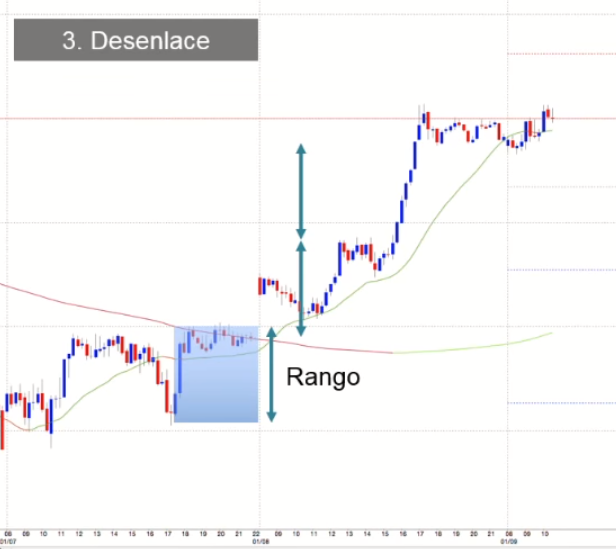
\includegraphics[scale=.65]{images/mod03-23.png}
    \end{center} 
    La zona sombrada es la bandera, el enfrentamiento del precio con la media móvil, y como, efectivamente, lo rompe, en la apertura del día siguiente del mercado el precio ya ha roto la media móvil y se ha situado por encima, para luego continuar su senda alcista, hasta llegar al nivel marcado. 

    Podemos ver cuál es la rentabilidad que habríamos obtenido en esta operación. El rango vendría determinado por la amplitud de la bandera, viendo que un rango y un poco más de dos, lo que indica que el beneficio podría estar un poco por encima de dos veces el rango, mientras que el \ti{stop loss} lo podríamos haber colocado como un porcentaje sobre el rango, por ejemplo del 20\%, o también podríamos colocarlo por debajo de los mínimos que marca el rango. En cualquier caso, el rato beneficio-riesgo habría sido muy favorable al obtener un beneficio mucho mayor que el riesgo soportado.
\end{itemize}

Aquí mostramos varios ejemplos de como en ocasiones la media móvil sirve como soporte par el precio, y la media móvil acaba rechazando el precio, llevándolo de nuevo a la tendencia primaria que tenía, que en este caso era alcista.
\begin{center}
    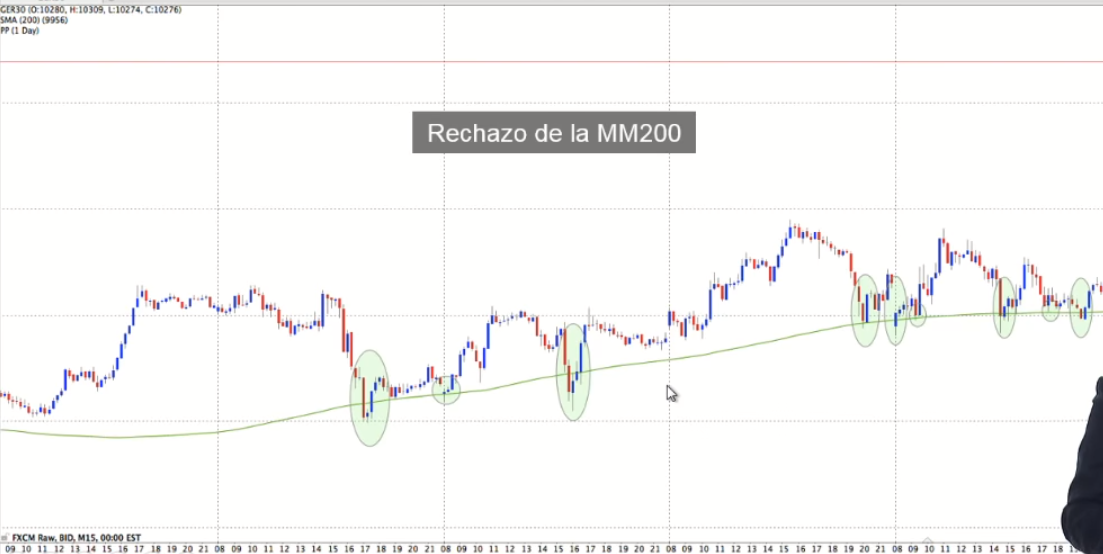
\includegraphics[scale=.65]{images/mod03-24.png}
\end{center} 
Vemos la media móvil de 200 períodos y el precio, también para el índice DAX-30, con el mismo \ti{time frame} de 15 minutos. ¿Qué observamos? el precio no llega a tocar la media móvil e incluso la llega a romper, durante quince minutos se situa por debajo de ésta, pero en la tercera vela reacciona hacia arriba y vuelve a la fase alcista. Vemos que hay períodos en los que ocurren situaciones similares. Cada uno de los puntos señalados en el gráfico generan señales de compra del activo, y todos ellos acabarían siendo provechosos, dando una rentabilidad positiva. 

De todos los puntos cabría señalar aquellos que rompen la media móvil hacia abajo, durante una o dos velas a lo sumo se quedan por debajo, pero es seguida de una reacción alcista que vuelve el precio por encima de la media móvil. Estas son señales inequivocas de que se deben tomar posiciones largas en el mercado.

A partir de este tipo de indicadores podemos montar una estrategia bursátil similar a la que habíamos analizado con la \ti{bandera}, y obteniendo una ratio rentabilidad-riesgo muy próximo al que veíamos.

\section{El análisis fundamental}

Hemos visto que el objetivo del análisis de las inversiones busca \tb{rentabilizar el capital}, ganar dinero de forma consistente y con un riesgo limitado.

Lo primero que piensa un inversor es qué activos voy a compra y cuáles voy a vender. Si hablamos de acciones existe un gran número de ellas en los mercados que se pueden comprar y vender. Una vez decidido que título compro puedo establecer a qué precio lo compro y a qué precio lo voy a vender para rentabilidar la inversión. Para todo esto son necesarios una serie de análisis que dependen de nuestro perfil inversor, inversor a largo plazo o a corto plazo.

Si somos un inversor a largo plazo, que quieran simplemente tener un dinero a la hora de la jubilación, uno de los análsis más recomendables es el \tb{análisis fundamental}. Este tipo de análisis nos permite realizar una serie de pronósticos, de expectativas, de la evolución a largo plazo de los activos. Se puede utilizar con cualquier tipo de activo, pero lo más común es hacerlo en relación con acciones cotizadas en bolsa.

¿En qué consiste el análisis fundamental?. Analiza aquellos activos, nos centramos en las acciones, que tienen un mayor potencial de revalorización, de tal forma que obtengamos rentabilidad tanto por el valor de la acción, que aumente con los años, como por los dividendos que nos va dando la empresa de los beneficios.

El análisis consiste en analizar la empresa en su totalidad. Existen diferentes tipos de análisis:
\begin{itemize}
    \item Pest 
    \item Dafo 
    \item Cadena de valor de Porter
\end{itemize}
en general, tratan de estudiar el entorno económico y los factores específicos de la empresa.
\begin{itemize}
    \item Entorno económico. Los efectos que pueden afectar a los beneficios de la empresa pueden ser:
    \begin{itemize}
        \item crecimiento del PIB 
        \item evolución de los tipos de interés, que permitan o dificulten que la empresa pueda financiarse.
        \item el tipo de cambio, influye en la competencia internacional.
    \end{itemize}
    \item Factores específicos de la empresa.
    \begin{itemize}
        \item Evolución de los ingresos,
        \item cartera de clientes,
        \item patentes, en el caso de empresas tecnológicas,
        \item competencia, etc.
    \end{itemize}
\end{itemize}

El problema que tenemos está en los \tb{datos}, éstos aparecen con una periodicidad anual, semestral o trimestral, pero no son datos que nos permitan estar controlando el precio de la acción a nivel diario; es decir, el análisis fundamental nos sirve para la especulación a corto plazo y es lo que hay que tener en consideración.

Dentro del análisis fundamental hay distintas estrategias, siendo las dos más importantes:

\begin{description}
    \item[Value investing], consiste en comparar el precio real con el valor teórico (información contable), que tienen en el mercado, en el momento actual, las acciones. Si vemos que el valor real difiere mucho del valor teórico, que el valor real es más bajo que el teórico, entonces interesa comprar las acciones, ya que pensamos que con el tiempo alcanzarán el valor teórico calculado, y obtendremos una rentabilidad conforme el valor se vaya acercando a nuestro valor teórico pues iremos vendiendo las acciones.
    
    Dentro de este análisis se pueden utilizar como indicadores de empresas que hay que analizar:
    \begin{itemize}
        \item Price Arning Ratio.
        \item Price to Book Ratio.
        \item así como otros ratios financieros económicos que nos indican cuál es la situación de la empresa.
    \end{itemize}

    \item[Grouth investing]. Se fija no en un valor teórico, en base a la información contable actual, sino en el potencial de crecimiento de las empresas. Es decir, localizo una empresa que pienso que en el futuro va a crecer muchísimo, y que tendrá mucho beneficio, lo que hará que sus acciones se revaloricen, que suban su precio.
    
    Aquí nos estamos basando en las \ti{expectativas}, pero hay que tener en cuenta, que muchas veces las expectativas están equivocadas, sobre todo si no hacemos nosotros mismos el análisis y nos fiamos del comportamiento general del mercado y demostramos un comportamiento gregario, hacemos lo que hacen los demás. Esto suele ocurrir cuando hay \ti{«burbujas»}, como ocurrió con la \ti{«burbuja tecnológica o inmobiliarias»}, donde hay mucha expectativa y todo el mundo apuesta por ellas, puede ocurrir que se hinche demasidado y finalmente explote.
\end{description}
